\documentclass[12pt]{article}
\title{Project 1}
\author{Eirik Ramsli Hauge\\
Joakim Kalsnes
}
\date{\today}

\usepackage{hyperref}
\usepackage{amsmath}
\usepackage[utf8]{inputenc}
\usepackage[english]{babel} 
%\usepackage{fullpage} 
\usepackage{amsfonts} 
\usepackage{amssymb} 
\usepackage{verbatim} 
 
\usepackage{color} 
\usepackage{setspace} 
\usepackage{blindtext}
\usepackage{epstopdf} 
\usepackage{braket}

\usepackage{cite} 
\usepackage{caption}
\usepackage{subcaption}
\usepackage{upgreek}
\usepackage{array,multirow}
\usepackage{pdfpages}

\usepackage{graphicx} 
\usepackage{float}

\usepackage{nameref}
\usepackage{hhline}
\usepackage{xtab}
\usepackage{booktabs, makecell, longtable}
\usepackage{lscape}

\newcommand{\E}[1]{\cdot 10^{#1}}
\newcommand{\e}[1]{\text{#1}}
\newcommand{\husk}[1]{\color{red} #1 \color{black}}


\DeclareMathOperator*{\argmin}{argmin}
\usepackage{bm}

\bibliographystyle{unsrt}

\begin{document}
\maketitle

\begin{abstract}
The aim of this project is to use ordinary least squared, Ridge and Lasso regression to learn about basic machine learning and how these algorithms work. We will create data with and without noise using the Franke Function and use each of the three methods to try and fit a polynomial to the data. Then we will import real map data and use the same methods again on this data. In the end we found that Ridge was the superior of the three methods, both with regards to accuracy and efficiency. The usage of bootstrap seemed to have little to no effect and we should have used k-fold as well to double check. 
\end{abstract}
\section{Introduction}   \label{s:i}
Although the theory behind machine learning has been known for a while, with modern computers the theories has had a renaissance. This is mostly due to the fact that we today have the computer power to efficiently use Machin Learning. The aim of this project is to look into three methods of regression analysis and compare them against each other. To do this we will write a script which uses both "home made" and premade functions from the python library \texttt{scikit learn}. These functions will then be applied to data from the Franke Function to learn more about them. Finally we will apply these methods to real map data and again compare each method to the other. The goal is that by the end we will have a better understanding of what works behind the black boxes of machine learning and why one is preferrable over the other in different situations.
\section{Theory} \label{s:t}
The following section follows closely the notation and derivation of linear models and the bootstrap in Hastie et al. chapter 3.2, 3.4 and 7.11. \cite{Hastie}.
\subsection{Linear regression}
In this project we will use different linear methods for regression. Linear regression is a linear approach to modelling the relationship between a response variable (also known as dependent variable) and one or multiple predictor (independent) variables. Given the input vector (predictor variables) $X^T = (X_1, X_2,...., X_p)$, a linear regression model predicts the output via the model
\begin{equation} \label{eq:lin_reg}
f(X) = \beta_{0} + \sum_{j=1}^{p}X_j\beta_{j}
\end{equation}
The $\beta_j$'s are unknown coefficients, and are what we are trying to estimate. The variables $X_j$ can come from different sources. They can for instance be quantitative inputs, transformations of the inputs or polynomials of the inputs such as $X_3 = X_2^2$ and $X_4 = X_1^2X_2$. No matter the source of the $X_j$, the model is linear in the parameters.
\subsubsection{Least squares method}
Let us say we have a set of training data $(x_1,y_1),....,(x_N,y_N)$ from which we want to estimate the parameters $\beta$. Each $x_i = (x_{i1},x_{i2},...,x_{ip})^T$ is a vector of measurements for the $i$th case. The least squares method chooses the coefficients $\beta = (\beta_0,\beta_1,...,beta_p)^T$ by minimizing the residual sum of squares
\begin{equation} \label{eq:least_squares}
\begin{split}
RRS(\beta) &= \sum_{i=1}^{N}(y_i-f(x_i))^2\\
&= \sum_{i=1}^{N}(y_i-\beta_0-\sum_{j=1}^{p}x_{ij}\beta_j)^2.
\end{split}
\end{equation}
If we denote by $\bm{X}$ the $N\times(p+1)$ matrix with each row an input vector (with a 1 in the first position), and let $\bm{y}$ be the N-vector of outputs in the training set, we can write the residual sum of squares as
\begin{equation}
RRS(\beta) = (\bm{y}-\bm{X}\beta)^T(\bm{y}-\bm{X}\beta).
\end{equation}
Differentiating with respect to $\beta$ gives
\begin{equation}
\frac{\partial RSS}{\partial \beta} = -2\bm{X}^T(\bm{y}-\bm{X}\beta)
\end{equation}
\begin{equation}
\frac{\partial^2RSS}{\partial \beta \partial \beta^T} = 2\bm{X}^T\bm{X}.
\end{equation}
We set the first derivative to zero (assuming that $\bm{X}$ has full column rank)
\begin{equation}
\bm{X}^T(\bm{y}-\bm{X}\beta) = 0
\end{equation}
to obtain the unique solution
\begin{equation}
\hat{\beta} = (\bm{X}^T\bm{X})^{-1}\bm{X}^T\bm{y}.
\end{equation}
This gives the predicted value at an input vector $x_0$ as $\hat{f}(x_0)=(1:x_0)^T\hat{\beta}$, and the fitted values at the training inputs:
\begin{equation}
\hat{\bm{y}}=\bm{X}\hat{\beta}=\bm{X}(\bm{X}^T\bm{X})^{-1}\bm{X}^T\bm{y},
\end{equation}
where $\hat{y_i}=\hat{f}(x_i)$.\\ \\

\subsubsection{R-squared, MSE, bias and variance}
The coefficient of determination, or R-squared ($R^2$), is a measure of the goodness of fit of a model. It is the proportion of the variance in the response variable that is predictable from the predictor variables, and hence takes a value between 0 and 1.\\
If we define $\bar{y}$ as the mean of the observed data,
\begin{equation}
\bar{y} = \frac{1}{N}\sum_{i=1}^{N}y_i,
\end{equation}
we can define $R^2$ using three sums of squares formulas:\\
1. Total sum of squares (proportional to the variance of the data)
\begin{equation}
SS_{tot} = \sum_{i=1}^{N}(y_i-\bar{y})^2
\end{equation}
2. The regression sum of squares (explained sum of squares)
\begin{equation}
SS_{reg} = \sum_{i=1}^{N}(\hat{f}(x_i)-\bar{y})^2
\end{equation}
3. The sum of squares of residuals
\begin{equation}
SS_{res} = \sum_{i=1}^{N}(y_i - \hat{f}(x_i))^2
\end{equation}
The most general definition of $R^2$ is then\\
\begin{equation}
R^2 := 1 - \frac{SS_{res}}{SS_{tot}}
\end{equation}
\\ \\

Another way of assessing the goodness of a model fit is by calculating the $mean\ squared\ error$ (MSE).
\begin{equation}
MSE = \frac{1}{N}\sum_{i=1}^{N}(y_i-\hat{f}(x_i))^2
\label{eq:MSE}
\end{equation}
This MSE can be decomposed into bias and variance.
\begin{equation}
\begin{split}
MSE &= E[(y-\hat{f}(x))^2] = Bias(\hat{f}(x))^2 + Var(\hat{f}(x)) + \sigma^2\\
&= (E[f(x)-\hat{f}(x)]^2) + (E[\hat{f}(x)^2]-E[\hat{f}(x)]^2) + \sigma^2
\end{split}
\end{equation}
The bias term measures how much the model, $\hat{f}(x)$, differs from the actual function, $f(x)$. A high bias means the model is underfitting the data. The model is not complex enough to capture all the information. On the other hand, a model can be overfitting. This happens when we use a very complex model that fits the training data very well. This model will have a high variance because it will be very sensitive to small fluctuations in the training set. As we can see, there is a trade-off between bias and variance. A simple model will have high bias and low variance, while a complex model will have low bias and high variance. The best model, i.e. lowest MSE, will be somewhere in the middle between a very simple and very complex model. In this project the bias and variance were calculated using the bootstrap technique (explained later).

\subsubsection{Shrinkage methods}
The least squares method is an intuitive and simple to understand-model, but the estimates obtained using this model are often not satisfactory. One of the reasons for this is the prediction accuracy. Least squares estimates often have low bias but large variance. By sacrificing a bit of bias to reduce the variance of the predicted values, the overall prediction accuracy may be improved. This can sometimes be done by setting some regression coefficients to zero or by shrinkage methods. Ridge regression and Lasso regression are examples of shrinkage methods.\\
Ridge regression shrinks the regression by imposing a penalty proportional to the square of the magnitude of the coefficients. To find the ridge coefficients, the penalized residual sum of squares is minimized.
\begin{equation}
\hat{\beta}^{ridge}=\argmin_{\beta}\{\sum_{i=1}^{N}(y_i-\beta_0-\sum_{j=1}^{p}x_{ij}\beta_j)^2+\lambda\sum_{j=1}^{p}\beta_j^2\}
\label{eq:ridge}
\end{equation}
The $\lambda\geq0$ parameter controls the amount of shrinkage, with increasing amount of shrinkage as $\lambda$ increases. A problem using the least squares method is that when there are many correlated predictor variables, their coefficients may become poorly determined and exhibit high variance. "A wildly large positive coefficient on one variable can be canceled by a similarly large negative coefficient on its correlated cousin." (Hastie p. 63). By imposing a penalty as in Ridge regression, this problem is reduced.\\
When performing a ridge regression it is common to use centered inputs. That is, each $x_{ij}$ is replaced by $x_{ij} - \bar{x}_j$. $\beta_0$ is estimated by $\bar{y}=\frac{1}{N}\sum_{1}^{N}y_i$, and the remaining coefficients get estimated by a ridge regression using centered inputs. We can write equation \ref{eq:ridge} in matrix form:\\
\begin{equation}
RSS(\lambda) = (\bm{y}-\bm{X}\beta)^T(\bm{y}-\bm{X}\beta)+\lambda\beta^T\beta.
\end{equation}
This gives the ridge regression solutions:
\begin{equation}
\hat{\beta}^{ridge} = (\bm{X}^T\bm{X}+\lambda\bm{I})^{-1}\bm{X}^T\bm{y},
\end{equation}
where $\bm{I}$ is the $p\times{p}$ identity matrix. By adding a positive constant to the diagonal of $\bm{X}^T\bm{X}$ before inversion the problem is made nonsingular, even if $\bm{X}^T\bm{X}$ is not of full rank.\\ \\
Another shrinkage method is the lasso. The lasso method is quite similar to ridge regression, but with some differences. We can write the lasso regression problem as
\begin{equation}
\hat{\beta}^{lasso}=\argmin_{\beta}\{\frac{1}{2}\sum_{i=1}^{N}(y_i-\beta_0-\sum_{j=1}^{p}x_{ij}\beta_j)^2+\lambda\sum_{j=1}^{p}\left|\beta_j\right|\}.
\label{eq:lasso}
\end{equation}
Equivalently, it can be written as
\begin{equation}
\begin{split}
\hat{\beta}^{lasso}=&\argmin_{\beta}\sum_{i=1}^{N}(y_i-\beta_0-\sum_{j=1}^{p}x_{ij}\beta_j)^2\\
&subject\ to\ \sum_{j=1}^{p}\left|\beta_j\right|\leq{t}.
\end{split}
\end{equation}
If $t$ is sufficiently small the nature of the constraint will cause some of the coefficients to be exactly zero. Thus, the lasso does a kind of continuous subset selection. The penalty parameter in both lasso and ridge regression should be chosen to minimize an estimate of the expected prediction error.\\
\subsubsection{Confidence intervals of $\beta$}
For ordinary least squared and ridge regression one can analytically find the confidence intervals of $\beta$. For ordinary least squared one finds the variance-covariance matrix by using the following formula:
\begin{equation}
\text{Var}(\beta) = (\bm{X}^T\bm{X})^{-1}\cdot \sigma^2
\end{equation}
where $\sigma^2$ is the estimated variance given by:
\begin{equation}
\sigma^2 = \frac{1}{N - p - 1} \sum\limits_{i=1}^N(y_i - \hat{y}_i)^2
\label{eqT:sigma2}
\end{equation}
The confidence interval is then given as $[\beta_j \pm 2\cdot std(\beta_j)]$ where we find $std(\beta_j)$ by taking the square root of diagonal elemnt $j$ in the variance-covariance matrix. \\ \\
Similarily, for ridge, the variance-covariance matrix is given by:
\begin{equation}
\text{Var}(\beta) = \sigma^2[\bm{X}^T\bm{X} + \lambda \bm{I}]^{-1}]\bm{X}^T\bm{X}([\bm{X}^T\bm{X} + \lambda I)^{-1})^T
\end{equation}
where we recognize all the elements from equations above. $\sigma^2$ is once again found from equation \eqref{eqT:sigma2} and the rest of the process is identical to the one above.
\subsection{Bootstrapping}
The bootstrap is a general tool used in statistics for assigning measures of accuracy to sample estimates. These measures of accuracy can for instance be defined in terms of bias, variance, prediction error or confidence intervals. Bootstrapping can be applied to a lot of statistical problems, e.g. hypothesis testing, model comparison and model optimization.\\
Say we have a model fit to a set of training data denoted by $\bm{Z}=(z_1,z_2,...,z_N)$ where $z_i = (x_i,y_i)$. The basic idea of the bootstrap is then to randomly draw datasets with replacement from the training set, where each sample has the same size as the original training set. This is done B times, producing B bootstrap datasets. For each bootstrap dataset we refit the model, and examine the behaviour of the quantities of interest. For instance the mean squared error, the r$^2$ score and the values of the $\beta$s can be computed for each dataset. This gives distributions of the quantities, and these distributions can be assessed by for instance mean and confidence intervals.
\subsection{Manipulating Data}
To test out different regression methods we will use the Franke Function defined \cite{Franke} as:
\begin{align*}
f(x,y) &= \frac{3}{4}\exp{\left(-\frac{(9x-2)^2}{4} - \frac{(9y-2)^2}{4}\right)}+\frac{3}{4}\exp{\left(-\frac{(9x+1)^2}{49}- \frac{(9y+1)}{10}\right)} \\
&+\frac{1}{2}\exp{\left(-\frac{(9x-7)^2}{4} - \frac{(9y-3)^2}{4}\right)} -\frac{1}{5}\exp{\left(-(9x-4)^2 - (9y-7)^2\right) }.
\end{align*}
Furthermore, we will sometimes want to add noise to this data. This will be done using the following formula:
\begin{equation*}
z = z + v \cdot N(n\_samples^2, 1)
\end{equation*}
where $z$ is the data from the Franke Function, $v$ is a variable $n\_samples^2$ is the same amount of rows as we have in $\bm{X}$ and $N$ gives the normal distribution \cite{Normal}.
\section{Experimental}   \label{s:e}
All scripts used in this project can be found on github at \url{https://github.com/eirikraha/fysstk3155---Project-1} in the \texttt{src} folder. By running the script named \texttt{taska.py} one must use one or two additional command line arguments. Each of these arguments will be described in turn below, but a brief summary is given in table \ref{tabE:sum}:
\begin{table}[H]
\centering
\begin{tabular}{c|p{12cm}}
\textbf{Arguments} & \textbf{Function} \\ \hline
a & Runs an ordinary least square regression analysis on the data produced by the Frankie Function. The data is also analyzed using bootstrap. \\ \hline
b & Runs a Ridge regression analysis on the data produced by the Frankie Function. The data is also analyzed using bootstrap. \\ \hline
b plot & Same as above, but one also produces a plot to visually determine the optimal $\lambda$. \\ \hline
b analyze & Same as "b", but one also produces two colorplots to visually determine the optimal $\lambda$ with regards to p and noise respectively. \\ \hline
c & Runs a Lasso regression analysis on the data produced by the Frankie Function. The data is also analyzed using bootstrap. \\ \hline
c plot & Same as above, but one also produces a plot to visually determine the optimal $\alpha$-value. \\ \hline
c analyze & Same as "c", but one also produces two colorplots to visually determine the optimal $\alpha$ with regards to p and noise respectively. \\ \hline
d & Imports map data from the file \texttt{SRTM\_data\_Norway\_1.tif} and plots the terrain data as a colormap in gray scale. \\ \hline
e & Imports map data from the file \texttt{SRTM\_data\_Norway\_1.tif} and divides the data into patches before performing ordinary least squared, ridge and lasso regression using bootstrap to find the optimal regression analysis. \\ \hline
e analyze & Does the same analyzis as the ones for "b plot/analyze". 
\end{tabular}
\caption{Summary of the different command line arguments accepted. One can also use the argument "all" to do every command line in succession.}
\label{tabE:sum}
\end{table}
The command line arguments a, b and c all represents different regression analysis as described in section \ref{s:t}. However, the script requires data to work upon. These data are produced by the Frankie Function where we give in two vectors, $\bm{x}$ and $\bm{y}$ and produce an array of z-values. The vectors  $\bm{x}$ and $\bm{y}$ are defined to be in the interval $\bm{x}, \bm{y} \in [0,1]$ and are uniformally distributed. Furthermore, one also needs the matrix $\bm{X}$ which contains all the functions we will allow the regression analysis to use in combination to recreate the data. For this project we will usually use combinations of $\bm{x}$ and $\bm{y}$ up to polynomials of fifth order.
\subsection{Command Line Argument: a}
Given the command line argument "a" the script will use the data from the Frankie Function and $\bm{X}$ to perform an ordinary least square regression analysis. This analysis is done on noise free and noisy data both by a home made function created using the linear algebra presented in section \ref{s:t} and using the LinearRegression function from \texttt{scikit learns}. The condifidence interval of $\beta$ is also found. Afterwards, R2 and MSE is calculated by the function \texttt{R2MSEeval} where one can choose to use either \texttt{scikit learns} or home made functions. Lastly, the script performs bootstrapping upon data with and without noise, evaluating for R2, MSE, bias and variance.
\subsection{Command Line Argument: b and c with or without plot or analyze}
The command line arguments "b" and "c" will do the same as "a" only using Ridge and Lasso regression respectively. If one adds the command line argument "plot" the script will produce plots of the R2 and MSE for different values of $\lambda$ and $\alpha$. These plots are then again used to finde the optimal and stable value for $\lambda$ and $\alpha$. For Lasso, one has to use the function provided from \texttt{scikit learn} as there is no home made function to be used. If one were to write the command line argument "analyze" the script will run through two different analyzis and produce colorplots. In the first the script compares different values of p (paramteres in $\bm{X}$) to different values of $\lambda$/$\alpha$. The second plot does the same only it compares different amount of noise to different values of $\lambda$/$\alpha$.   
\subsection{Command Line Argument: d}
This command line argument provides a part of the script which is more used as a proof of concept. By providing "d" as your argument, the class \texttt{terrainReader} will import the map data stored in the file \texttt{SRTM\_data\_Norway\_1.tif} and plot it. This is a general method which can be used for all \texttt{.tif}-files downloaded from \url{https://earthexplorer.usgs.gov/}.
\subsection{Command Line Argument: e with or without analyze}
Lastly, the commmand line argument "e" will provide you with a combination of all the tasked performed previously. The script will now read the map data, divide it into a set number of patches and perform ordinary least square, ridge and lasso regression using bootstrap. The MSE, R2, bias and variance will then be calculated for each method. Choosing the command line argument "analyze" at the end one will perform the same type of analyzis as if one were to choose "plot" and "analyze" for "b" and "c".

\section{Results and Discussion}  \label{s:rd}
All results which are either written to file or plotted can be found in the \texttt{benchmarks} and \texttt{figures} folders. \\ \\
Before we can actively use Ridge and Lasso regression, we need to find the optimal $\lambda$ and $\alpha$ value. To perform an analyzis upon this, we use the "b"/"c" and "plot" or "analyze" command line arguments. Using the "plot" argument will provide the plots presented in figure \ref{figRD:RLR2MSE}:
\begin{figure}[H]
\centering
\begin{subfigure}[t]{0.48\textwidth}
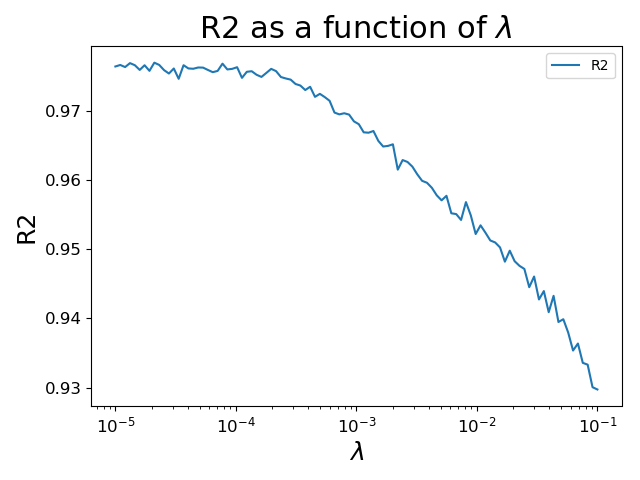
\includegraphics[width=\linewidth]{../figures/RidgeR2.png}
\caption{Ridge R2}
\label{figRD:RR2}
\end{subfigure}
\ \
\begin{subfigure}[t]{0.48\textwidth}
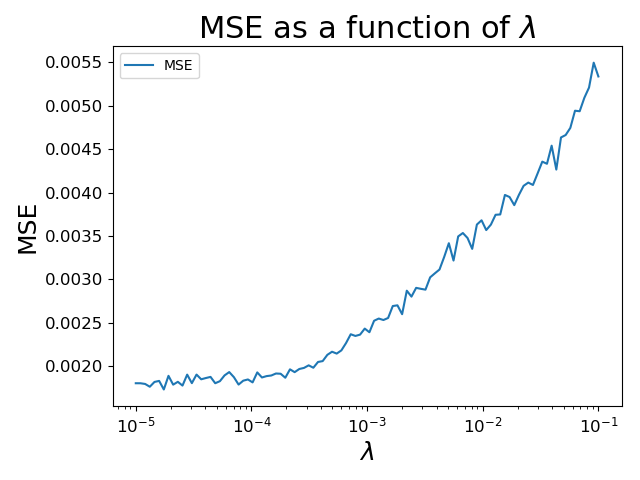
\includegraphics[width = \linewidth]{../figures/RidgeMSE.png}
\caption{Ridge MSE}
\label{figRD:RMSE}
\end{subfigure}
\\
\begin{subfigure}[t]{0.48\textwidth}
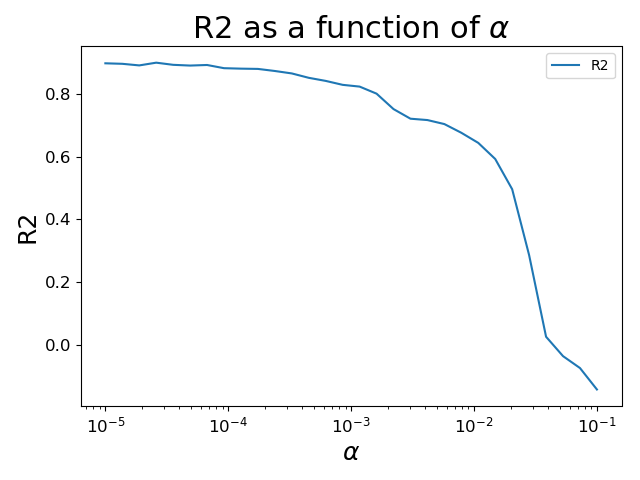
\includegraphics[width=\linewidth]{../figures/LassoR2.png}
\caption{Lasso R2}
\label{figRD:LR2}
\end{subfigure}
\
\begin{subfigure}[t]{0.48\textwidth}
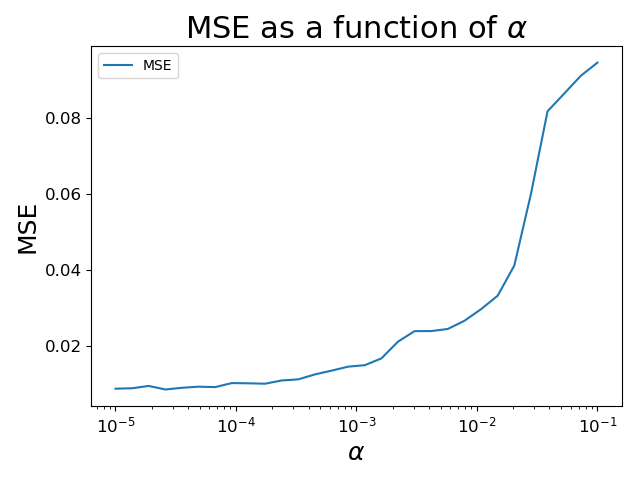
\includegraphics[width = \linewidth]{../figures/LassoMSE.png}
\caption{Lasso MSE}
\label{figRD:LMSE}
\end{subfigure}
\caption{R2-scores and MSE for different values of $\lambda$ and $\alpha$ using Ridge and Lasso respectively.}
\label{figRD:RLR2MSE}
\end{figure}
Figure \ref{figRD:RLR2MSE} indicates that for both $\lambda$ and $\alpha$ the quality of our predicted function declines after about $1\E{-4}$ while it stays relatively constant prior to this value. \\ \\
Furthermore, using the "analyze" argument produced the plots presented in figure \ref{figRD:colorRidgeP}, figure \ref{figRD:colorLassoP},\ref{figRD:colorRidgeN} and figure \ref{figRD:colorLassoN}:
\begin{figure}[H]
\centering
\begin{subfigure}[t]{0.98\textwidth}
\includegraphics[width=\linewidth]{../figures/{Ridge-p-10.00-R2-mini0.70-maxi1.00}.png}
\caption{R2}
\label{figRD:cpRR2}
\end{subfigure}
\\
\begin{subfigure}[t]{0.98\textwidth}
\includegraphics[width = \linewidth]{../figures/{Ridge-p-10.00-MSE-mini0.00-maxi0.02}.png}
\caption{MSE}
\label{figRD:cpRMSE}
\end{subfigure}
\caption{Colorplot of MSE and R2 as a function of p and $\lambda$}
\label{figRD:colorRidgeP}
\end{figure}

\begin{figure}[H]
\centering
\begin{subfigure}[t]{0.98\textwidth}
\includegraphics[width=\linewidth]{../figures/{Lasso-p-6.00-R2-mini0.70-maxi1.00}.png}
\caption{R2}
\label{figRD:cpLR2}
\end{subfigure}
\\
\begin{subfigure}[t]{0.98\textwidth}
\includegraphics[width = \linewidth]{../figures/{Lasso-p-6.00-MSE-mini0.00-maxi0.02}.png}
\caption{MSE}
\label{figRD:cpLMSE}
\end{subfigure}
\caption{Colorplot of MSE and R2 as a function of p and $\alpha$}
\label{figRD:colorLassoP}
\end{figure}

From figures \ref{figRD:colorRidgeP} and figure \ref{figRD:colorLassoP} we can see that increasing p while decreasing $\lambda$/$\alpha$ is a good approach to achieve better results. However, we can also observe that beyond a certain point there is little use in increasing P or decreasing $\lambda$/$\alpha$. Since doing this also will increase computation time, it is wise to find the lowest P and highest $\lambda$/$\alpha$ which gives adequate results. As we can see P = 5 and $\lambda$/$\alpha = 1\E{-4}$ does preciesly this. It could be argued to be increased even more, but then we would also be apt to overfitting the function. \\ \\
By analyzing the noise, we see the same trend. These plots can be viewed in figure \ref{figRD:colorRidgeN} and figure \ref{figRD:colorLassoN} in appendix A. It is clear to see that by increasing the noise, we can see that we need a sufficient low $\lambda$/$\alpha$ to achieve the optimal results. Once again, we wish to find the lowest value which gives adequate results and one can once again argue that $1\E{-4}$ is a good value for both $\lambda$ and $\alpha$. \\ \\ \\
Given the analyzis above, we can find a fit to our Franke Function using ordinary least squared, Ridge and Lasso regression. The results can be found in table \ref{tabRD:abc}.

\begin{table}[H]
\centering
\begin{tabular}{c|c|c|c|c|c|c}
Method & R2 & MSE & $\lambda$ /$\alpha$ & Variance & Bias & Error \\ \hline
OLS & $0.98$ & $1.91\E{-3}$ & -  & - & - & -  \\ \hline
Ridge & $0.98$ & $1.82\E{-3}$ & $1\E{-4}$ & - & - & -  \\ \hline
Lasso & $0.89$ & $9.54\E{-3}$ & $1\E{-4}$ & - & - & -  \\ \hline
OLS* & $0.98$ & $1.91\E{-3}$ & - & - & - & -  \\ \hline
Ridge* &  $0.98$ & $1.82e-03$ & $1\E{-4}$ & - & - & -  \\ \hline
Lasso* &$0.89$ & $9.55\E{-3}$ & $1\E{-4}$ & - & - & -  \\ \hline
OLS$^{\dagger}$ & $0.98$ & $1.90\E{-3}$ & - & $9.62\E{-6}$ & $1.89\E{-3}$ & $1.90\E{-3}$ \\ \hline
Ridge$^{\dagger}$ & $0.98$ & $1.91\E{-3}$ & $1\E{-4}$ & $8.44\E{-6}$ & $1.90\E{-3}$ & $1.91\E{-3}$  \\ \hline
Lasso$^{\dagger}$ & $0.89$ & $9.36\E{-3}$ & $1\E{-4}$ & $1.49\E{-5}$ & $9.34\E{-3}$ & $9.36\E{-3}$   \\ \hline
\end{tabular}
\caption{Results from OLS, Ridge and Lasso regression on data from the Franke Function, data from the Franke Function with added noise of 0.01 (*) and by using bootstrap with 1000 iterations ($\dagger$). - symbolises values not relevant or nonexisting.}
\label{tabRD:abc}
\end{table}
As we can see there are small differences between ordinary least squared and Ridge, however Lasso seems to be the biggest looser. It is evident that the noise contribution is too small to make any difference and should be increased for a more in depth study of its effect. By bootstrapping we can see that the R2-score and MSE are relatively stable. The bias and variance have big differences for all three methods with Bias being the main contributor to the error. This effect is less prominent for Lasso as is to be expected. In fact, the difference should be bigger and it might seem that we overfit the Lasso. It is also worth to notice that the scores are roughly the same for both ordinary methods and with the use of bootstrap. As bootstrap aims to assign more accuracy, we must conclude that the original measurements were quite accurate. This, however, seems odd and bootstrap should improve on our measurements. Why this is not evident here, is something one should look into in future studies. In the future, we would use k-fold validation instead of bootstrap to see if we achieve similar results.\\ \\
Given these analyzis it seems as though Ridge is the optimal method. With both low errors and a high R2-score this method seems to be the obvious choice. There seems to be something off with our Lasso and probably the scores found for this method should be higher. This could possible be caused by a too high $\alpha$-value. However, the Lasso method is much more time consuming than the Ridge method and therefore we will deem the Ridge method to be the superior one even if we were able to produce the same results with Lasso. \\ \\
The confidence intervals of $\beta$ are presented for ordinary least squared and ridge in figure \ref{figRD:conf}. As we can see, something has gone horrible wrong for the ridge $\beta$'s. Due to time constraints we are not able to do anything about it, but for future works we would look into this function. Most likely there is something wrong in our theory for finding these confidence intervals.
\begin{figure}[H]
\centering
\begin{subfigure}[t]{0.48\textwidth}
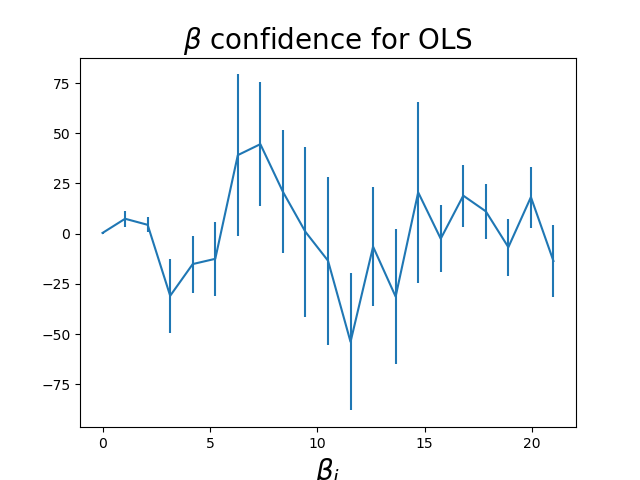
\includegraphics[width=\linewidth]{../figures/a-OLS-contour-beta-patchNone.png}
\caption{OLS}
\label{figRD:OLSconf}
\end{subfigure}
\ \
\begin{subfigure}[t]{0.48\textwidth}
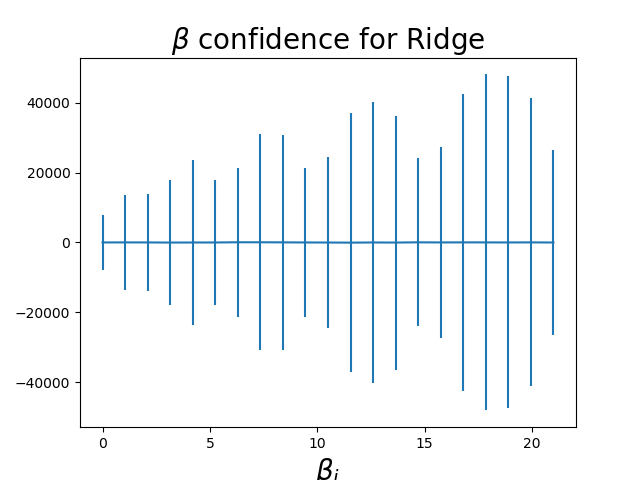
\includegraphics[width = \linewidth]{../figures/b-Ridge-contour-beta-patchNone.png}
\caption{Ridge}
\label{figRD:Rconf}
\end{subfigure}
\caption{Confidence intervals for $\beta$'s found for both ordinary least square and ridge.}
\label{figRD:conf}
\end{figure}
Because of the size of the data provided from the file \texttt{SRTM$\_$data$\_$Norway\_1.tif} we chose to divide the set into ten parts. Due to that we wished to make each patch equal in size, we lost some of the data from the original file. However, this is not crucial as the principle we are to look into remains the same. Because of this, most calculations to find optimal values were carried out upon just one patch of data to save time. We assumed that each patch of data is roughly as varied in terrain as the next and thus we assumed that what is best for one patch is best for all. However, this assumption may not hold up in the end, but it will hopefully give a good estimation. \\ \\
Doing the same analyzis as above to find the optimial $\lambda$ and $\alpha$, one recieves similar plots and can find that an optimal value lies between $1\E{-4}$ and $1\E{-3}$. The figures can be found in appendix A. \\ \\
Once again we wanted to see the confidence interval of $\beta$, and once again the Ridge interval failed us. The confidence interval for ordinary least squared can be found in figure \ref{figRD:confe}
\begin{figure}[H]
\centering
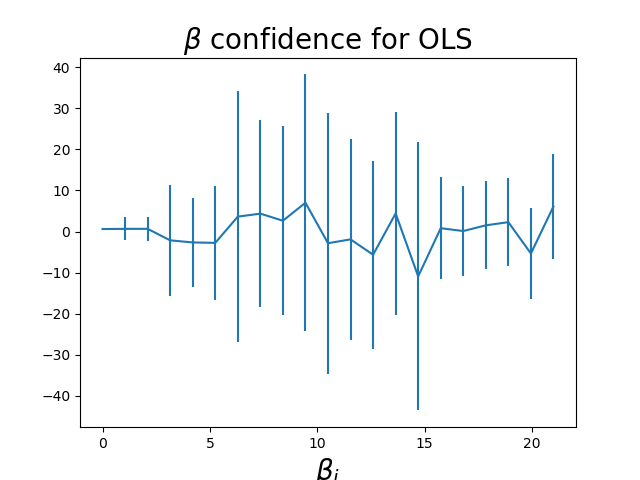
\includegraphics[scale=0.5]{../figures/e-OLS-contour-beta-patch0.png}
\caption{$\beta$-values and confidence intervals for OLS of patch 1.}
\label{figRD:confe}
\end{figure}
Using $\lambda = \alpha = 1\E{-4}$ we found the values presented in table \ref{tabRD:e} using bootstrap with the three different regression methods.
\begin{table}[H]
\centering
\begin{tabular}{c|c|c|c|c|c|c|c}
Patch & Method & R2 & MSE & $\lambda$ /$\alpha$ & Variance & Bias & Error \\ \hline
\multirow{3}{*}{Patch 1} & OLS & $0.97$ & $2.26\E{-4}$ & - & $5.50\E{-7}$ & $2.25\E{-4}$ & $2.26\E{-4}$ \\ \cline{2-8}
& Ridge & $0.97$ & $2.26\E{-4}$ & $1.00\E{-4}$ & $5.20\E{-7}$ & $2.25\E{-4}$ & $2.26\E{-4}$  \\ \cline{2-8}
& Lasso & $0.90$ & $7.65\E{-4}$ & $1.00\E{-4}$ & $1.06\E{-6}$ & $7.64\E{-4}$ & $7.65\E{-4}$\\ \hline
\multirow{3}{*}{Patch 5} & OLS & $0.83$ & $2.32\E{-4}$ & - & $5.67\E{-7}$ & $2.32\E{-4}$ & $2.32\E{-4}$  \\ \cline{2-8}
& Ridge & $0.82$ & $2.39\E{-4}$ & $1.00\E{-4}$ & $5.45\E{-7}$ & $2.39\E{-4}$ & $2.39\E{-4}$  \\ \cline{2-8}
& Lasso & $0.52$ & $6.57\E{-4}$ & $1.00\E{-4}$ & $8.63\E{-7}$ & $6.56\E{-4}$ & $6.57\E{-4}$ \\ \hline
\multirow{3}{*}{Patch 10} & OLS & $0.90$ & $6.97\E{-4}$ & - & $2.07\E{-6}$ & $6.95\E{-4}$ & $6.97\E{-4}$ \\ \cline{2-8}
& Ridge & $0.90$ & $6.71\E{-4}$ & $1.00\E{-4}$ & $2.05\E{-6}$ & $6.69\E{-4}$ & $6.71\E{-4}$ \\ \cline{2-8}
& Lasso & $0.71$ & $1.97\E{-3}$ & $1.00\E{-4}$ & $2.68\E{-6}$ & $1.97\E{-3}$ & $1.97\E{-3}$  \\ \hline
\multirow{3}{*}{Patch 15} & OLS & $0.96$ & $3.24\E{-4}$ & - & $7.31\E{-7}$ & $3.23\E{-4}$ & $3.24\E{-4}$ \\ \cline{2-8}
& Ridge & $0.96$ & $3.27\E{-4}$ & $1.00\E{-4}$ & $7.15\E{-7}$ & $3.26\E{-4}$ & $3.27\E{-4}$\\ \cline{2-8}
& Lasso & $0.93$ & $5.45\E{-4}$ & $1.00\E{-4}$ & $5.16\E{-7}$ & $5.44\E{-4}$ & $5.45\E{-4}$ \\ \hline
\multirow{3}{*}{Patch 20} & OLS & $0.84$ & $3.89\E{-4}$ & - & $8.57\E{-7}$ & $3.88\E{-4}$ & $3.89\E{-4}$ \\ \cline{2-8}
& Ridge & $0.83$ & $4.07\E{-4}$ & $1.00\E{-4}$ & $8.05\E{-7}$ & $4.07\E{-4}$ & $4.07\E{-4}$ \\ \cline{2-8}
& Lasso & $0.66$ & $8.13\E{-4}$ & $1.00\E{-4}$ & $7.38\E{-7}$ & $8.12\E{-4}$ & $8.13\E{-4}$ \\ \hline
\end{tabular}
\caption{Results from OLS, Ridge and Lasso regression on data from the real map data by using bootstrap with 1000 iterations. - symbolises values not relevant or nonexisting. Only five patches where chosen as they are thought to represent all the data. For all patches, please see the benchmarksfile \texttt{taske.txt}.}
\label{tabRD:e}
\end{table}
From table \ref{tabRD:e} it is evident that there are differences within each patch as to how well our model fits. As the $\alpha$ and $\lambda$ values are fitted to patch 1, it is only natural that this patch scores high. However, the highest scoring patch is patch 15. It seems as though the regression methods we have used are all quite good at representing real map data in some cases, however, in others they seem to fall short. Ideally we would fine tune the models for each patch so that in the end they all had good results, but that requires more time and is left for future projects. It would have been better to treat all of the map data at once instead of dividing it up into 20 patches, but this would also lead to bias towards the more common data points as the ones that don't "fit in" would be ignored. If many of these points are in one patch, the different methods fine tuned to each patch will be better. \\ \\
We can see that what we found in table \ref{tabRD:abc} seems to hold true. Ordinary least squared and Ridge seems to be the superior models while Lasso seems to fall a bit behind. Once again, this seems a bit odd, but as it happens again and again, it is most likely caused by something in the script rather than faults in the data. \\
Given that these data most likely already contians noise, no noise evaluation was performed. \\ \\
For future projects we would recommend looking further into Lasso, making it more accurate. We would also recommend trying different map datas from around the world to see if the same analysis holds true. It would also be preferrable with a computer powerful enough to treat large maps and we would recommend parallell processing to make Bootstrap more efficient. On the same note, we would also recommend adding k-fold validation to further analyze the data alongside bootstrap. 
\section{Conclusion}  \label{s:con}
We have found that for both the data from the Franke Function and the data from maps that the Ridge method is the superior method with regards to efficiency, R2 and MSE. Something seems a bit off with our Lasso and it would possible give better results if one found a better $\alpha$-value. For future works one should invest more time in finding good $\lambda$ and $\alpha$-values and do more iterations in each bootstrap. One should also do a more in depth analysis of whether or not the functions are over/underfitted.
\section*{References} \label{s:ref}
\bibliography{references}
\section*{Appendix A} \label{app:A}
\begin{figure}[H]
\centering
\begin{subfigure}[t]{0.98\textwidth}
\includegraphics[width=\linewidth]{../figures/{Ridge-noise-0.30-R2-mini0.70-maxi1.00}.png}
\caption{R2}
\label{figRD:cnRR2}
\end{subfigure}
\\
\begin{subfigure}[t]{0.98\textwidth}
\includegraphics[width = \linewidth]{../figures/{Ridge-noise-0.30-MSE-mini0.00-maxi0.02}.png}
\caption{MSE}
\label{figRD:cnRMSE}
\end{subfigure}
\caption{Colorplot of MSE and R2 as a function of noise and $\lambda$}
\label{figRD:colorRidgeN}
\end{figure}

\begin{figure}[H]
\centering
\begin{subfigure}[t]{0.98\textwidth}
\includegraphics[width=\linewidth]{../figures/{Lasso-noise-0.30-R2-mini0.70-maxi1.00}.png}
\caption{R2}
\label{figRD:cnLR2}
\end{subfigure}
\\
\begin{subfigure}[t]{0.98\textwidth}
\includegraphics[width = \linewidth]{../figures/{Lasso-noise-0.30-MSE-mini0.00-maxi0.02}.png}
\caption{MSE}
\label{figRD:cnLMSE}
\end{subfigure}
\caption{Colorplot of MSE and R2 as a function of noise and $\alpha$}
\label{figRD:colorLassoN}
\end{figure}

\begin{figure}[H]
\centering
\begin{subfigure}[t]{0.48\textwidth}
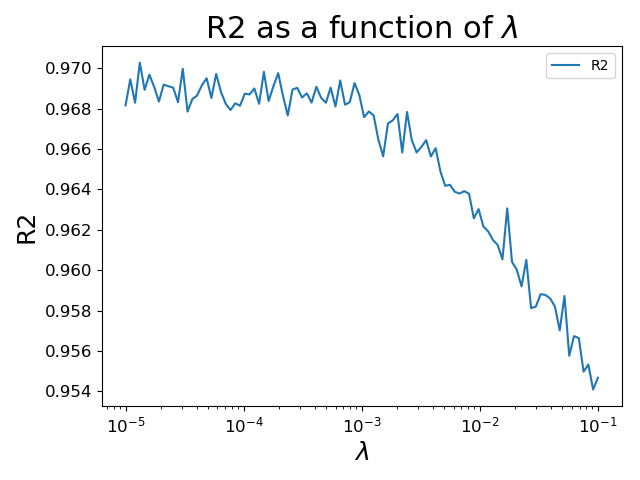
\includegraphics[width=\linewidth]{../figures/Taske_RidgeR2.png}
\caption{Ridge R2}
\label{figRD:RR2}
\end{subfigure}
\ \
\begin{subfigure}[t]{0.48\textwidth}
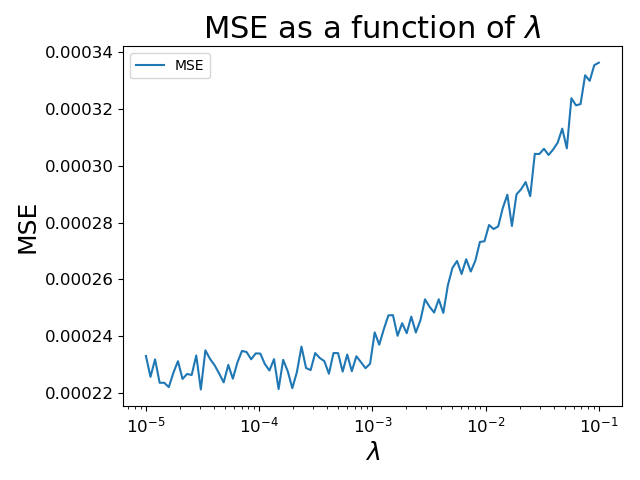
\includegraphics[width = \linewidth]{../figures/Taske_RidgeMSE.png}
\caption{Ridge MSE}
\label{figRD:RMSE}
\end{subfigure}
\\
\begin{subfigure}[t]{0.48\textwidth}
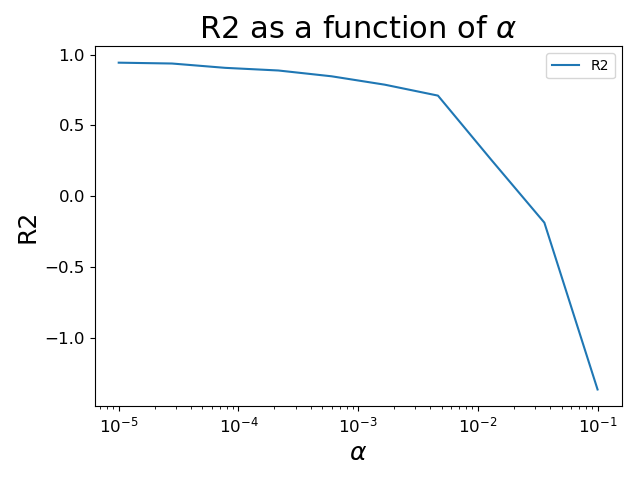
\includegraphics[width=\linewidth]{../figures/Taske_LassoR2.png}
\caption{Lasso R2}
\label{figRD:LR2}
\end{subfigure}
\
\begin{subfigure}[t]{0.48\textwidth}
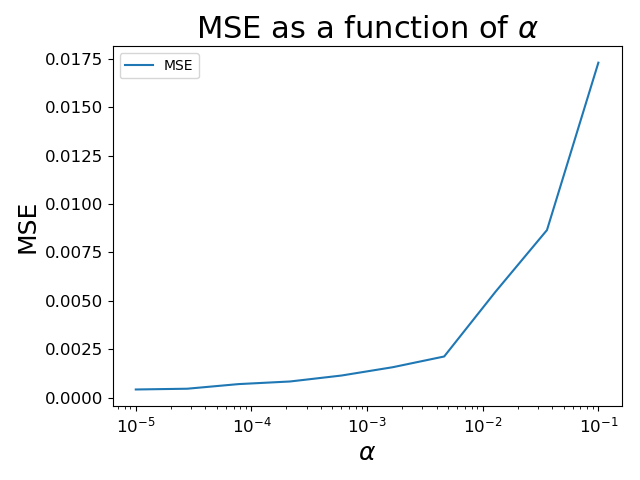
\includegraphics[width = \linewidth]{../figures/Taske_LassoMSE.png}
\caption{Lasso MSE}
\label{figRD:LMSE}
\end{subfigure}
\caption{R2-scores and MSE for different values of $\lambda$ and $\alpha$ using Ridge and Lasso respectively upon data from patch 1.}
\label{figRD:RLR2MSE}
\end{figure}


\begin{figure}[H]
\centering
\begin{subfigure}[t]{0.98\textwidth}
\includegraphics[width=\linewidth]{../figures/{Taske_Ridge-p-6.00-R2-mini0.70-maxi1.00}.png}
\caption{R2}
\label{figRD:cpRR2}
\end{subfigure}
\\
\begin{subfigure}[t]{0.98\textwidth}
\includegraphics[width = \linewidth]{../figures/{Taske_Ridge-p-6.00-MSE-mini0.00-maxi0.02}.png}
\caption{MSE}
\label{figA:cpRMSE}
\end{subfigure}
\caption{Colorplot of MSE and R2 as a function of p and $\lambda$ for patch 1}
\label{figA:colorRidgeP}
\end{figure}

\begin{figure}[H]
\centering
\begin{subfigure}[t]{0.98\textwidth}
\includegraphics[width=\linewidth]{../figures/{Taske_Lasso-p-6.00-R2-mini0.70-maxi1.00}.png}
\caption{R2}
\label{figA:cpLR2}
\end{subfigure}
\\
\begin{subfigure}[t]{0.98\textwidth}
\includegraphics[width = \linewidth]{../figures/{Taske_Lasso-p-6.00-MSE-mini0.00-maxi0.02}.png}
\caption{MSE}
\label{figA:cpLMSE}
\end{subfigure}
\caption{Colorplot of MSE and R2 as a function of p and $\alpha$ for patch 1}
\label{figA:colorLassoP}
\end{figure}

\end{document}